\chapter{Simulation of Reconstruction Algorithm}
This chapter will describe how the system can be mathematically modelled and how the mask for the lensless imager was designed. As mentioned in the previous chapter the system can be modelled as 
\begin{equation}
\label{eq:conv2}
y = \phi * x + e ;
\end{equation}
Ignoring the noise and converting the equation to fourier domain, the equation \ref{eq:conv2} can be re-written as
\begin{equation}
\label{eq:conv3}
F(y) = F(\phi)F(x)
\end{equation}
\begin{equation}
\label{eq:conv3}
F(x) = \frac{F(y)}{F(\phi)}
\end{equation}
\begin{equation}
\label{eq:conv4}
x = F^{-1}(\frac{F(y)}{F(\phi)})
\end{equation}
Equation \ref{eq:conv4} is the simplest possible computational inversion of the scene from the sensor. This method has also been used in \cite{Toeplitz}. As mentioned in the previous chapter, there are two types of masks that can be used for the purpose of encoding the scene onto the mask, namely separable and non-separable mask. MATLAB has been used for the purpose of simulating the algorithms. In this chapter, we would simulate two types of mask patterns, namely separable and non-separable mask patterns. A separable mask pattern is one in which the mask matrix $\phi$ can be expressed in-terms of two sub- matrices:
\begin{equation}
\phi = \phi_L * \phi_R
\end{equation}
Both $\phi_L$ and $\phi_R$ are doubly-toeplitz mask. The mathematical model is also changed as described by the equation \ref{eq:separable}. A non-separable mask is one which does not follow this property and follows equation \ref{eq:conv2}.

\section{Simulation of a non-separable mask}
The non-separable mask simulation was carried out as shown in Figure \ref{fig:non_sep_sim}.

\begin{figure}[ht]
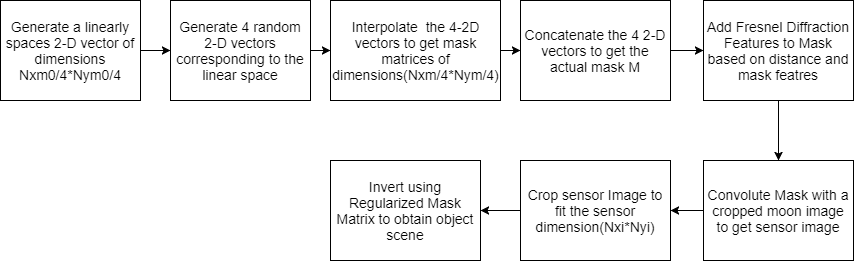
\includegraphics[scale = 0.50]{pics/non_sep_sim_flow}
\caption{Simulation-Flow non-separable matrix}
\label{fig:non_sep_sim}
\end{figure}
\section{Simulation of a separable mask}